\chapter{Funktio}

Matematiikassa tutkitaan usein asioiden välisiä riippuvuuksia. Tällaiset riippuvuudet voidaan muotoilla funktioiden avulla. Esimerkiksi lukiolaisen käytössä oleva rahan määrä voisi olla ajan $t$ funktio $f(t)$.  Varmaankin $f(t)$ 
hyppäisi ylöspäin hetkellä $t$, jolloin viikkorahat maksetaan ja sitten se laskisi tasaisesti (tai epätasaisesti), kunnes viikkoraha maksetaan seuraavan kerran.  Jos $f(t)$ on negatiivinen, niin se tarkoittaa, että lukiolaisellamme on hetkellä $t$ velkaa.

\laatikko{\emph{Funktiolla} $f(x)$ tarkoitetaan \emph{sääntöä}, joka liittää \emph{muuttujaan} $x$ arvon $y=f(x)$.

Tarkemmin funktioon liittyy \emph{määrittelyjoukko} $A$, johon muuttuja $x$ kuuluu, \emph{arvojoukko} $B$, johon funktion arvot kuuluvat ja sääntö
$y=f(x)$, joka liittää jokaiseen määrittelyjoukon $A$:n alkioon $x$ arvojoukon $B$ alkion $y$.}

\begin{esimerkki}
Määritellään funktio $f$ tavaroiden joukolta $A$ reaaliluvuille joka kuvaa jokaisen tavaran sen arvonlisäveroprosentille.
\[A = \{\text{ahvenfilee}, \text{AIV-rehu}, \text{auto}, \text{runokirja}, \text{ravintola-ateria}, \text{särkylääke}, \text{televisio}\}\]
[Selitys arvonlisäverokannoista ja $f(\text{ahvenfilee}) = 13$, $f(\text{AIV-rehu}) = 13$, $f(\text{auto}) = 23$, $f(\text{runokirja}) = 9$, $f(\text{ravintola-ateria}) = 13$, $f(\text{särkylääke}) = 9$, $f(\text{televisio}) = 23$]
\begin{center}
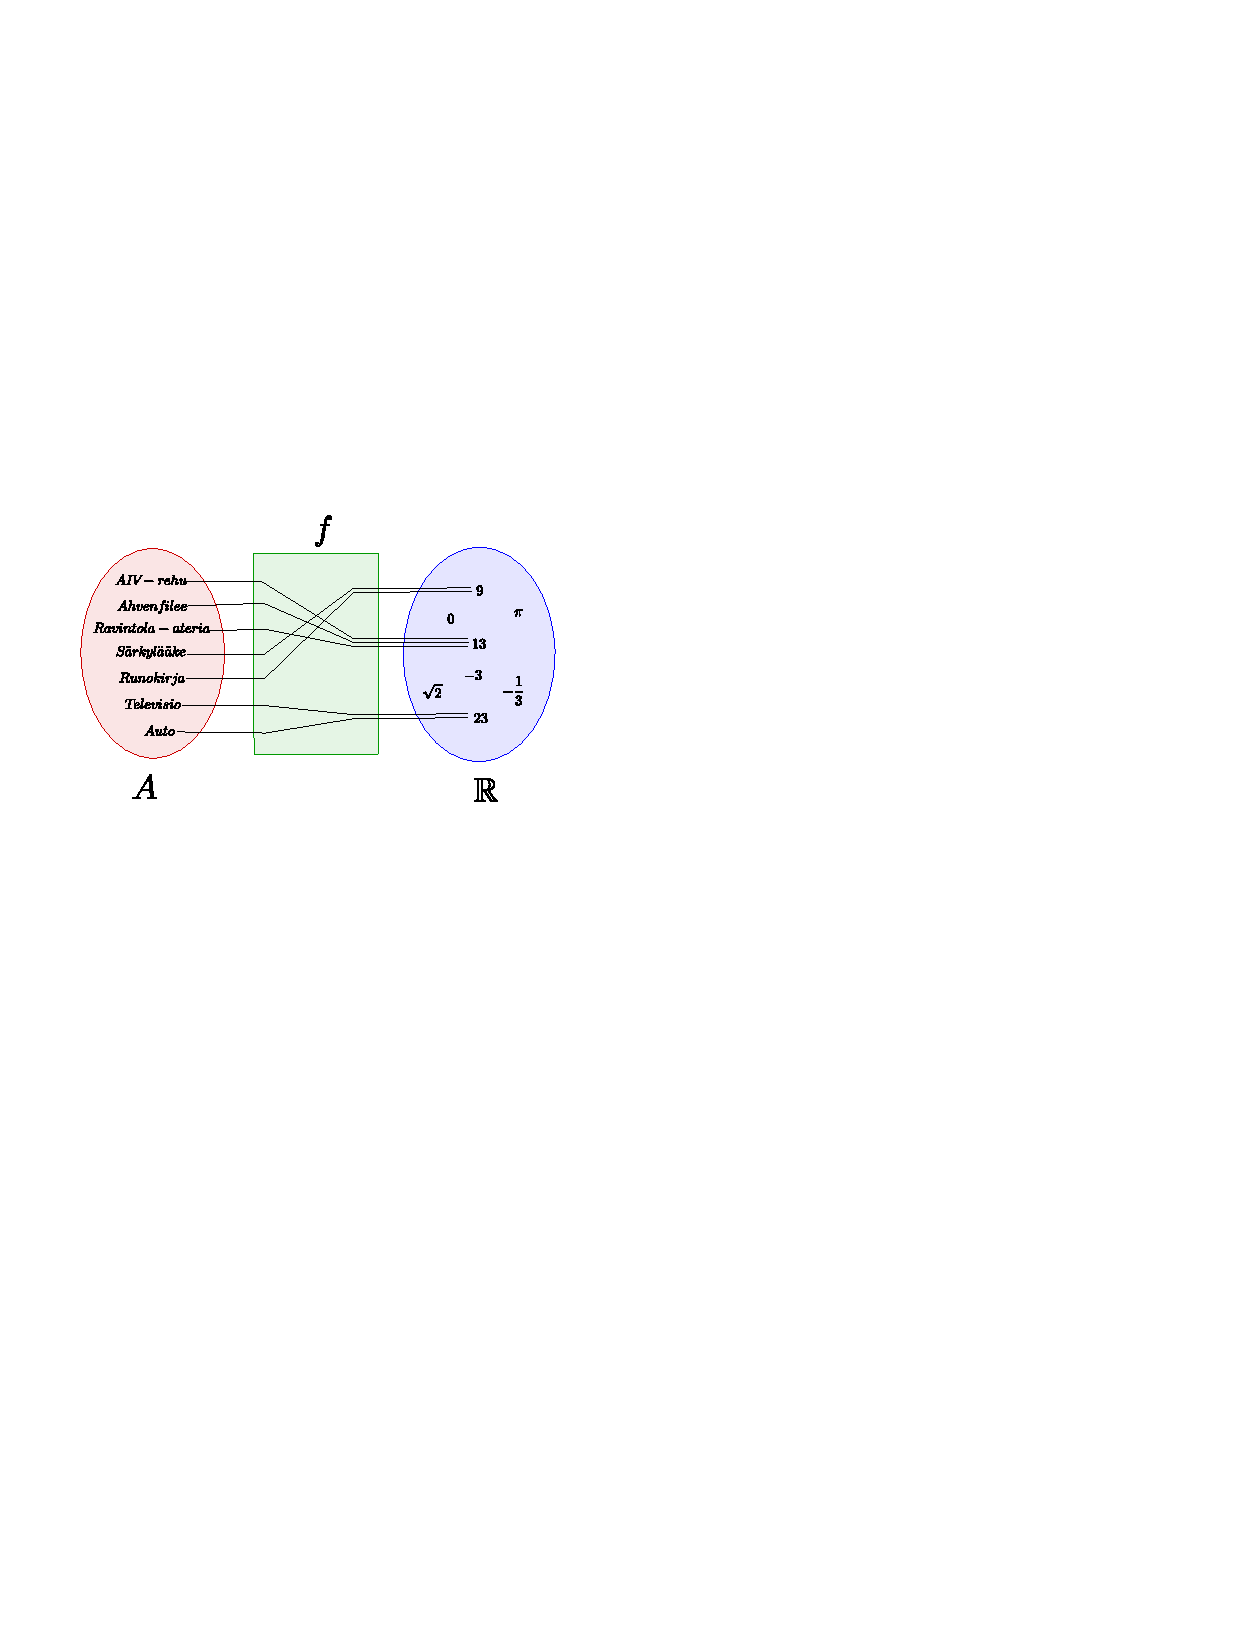
\includegraphics[width=13cm]{03-funktiot/kuvia/funktiokone.pdf}
\end{center}
\end{esimerkki}

\missingfigure{Klassinen funktiokuva $f:A\to B$, jossa nuolen päällä merkintä $f(x)=y$.}

Käytäntöjä:
\begin{itemize}
\item $f(x) = y$ lausutaan: "Funktio saa arvon $y$ pisteessä $x$."
\item Funktion määrittely- ja maalijoukot jätetään usein merkitsemättä, jos ne ovat selviä asiayhteydestä. Tällä kurssilla maalijoukko on yleensä reaaliluvut.
\item Funktion sääntöä kutsutaan usein pelkästään funktioksi.
\item Joskus funktio samaistetaan sen kuvaajan kanssa.  Siis sääntö $y=f(x)$ samaistetaan $xy$-koordinaatison käyrää.
\end{itemize}

\begin{esimerkki}
Leena Lukiolainen saa kuukausirahaa $100$ euroa.  Kuukausiraha maksetaan kuun lopussa. Tämän lisäksi kesä-, heinä- ja elokuussa Leena on töissä Siperian Wallinnassa.  Leenan kuukausipalkka kesätöissä on $1\ 500$ euroa ja palkka maksetaan kuun lopussa.  Mitään muita tuloja Leenalla ei ole, eikä Leena kuluta rahojaan ollenkaan, vaan panee ne sukanvarteen tulevia opintoja varten. 

Tarkastelemme Leenan varallisuuden kehittymistä vuoden aikana ajan $t$ funktiona. Määrittelyjoukko $A$ on siis vuosi. Laskemme aikaa $t$ kuukausina (ja yksinkertaisuuden vuoksi oletamme, että kuukaudet ovat saman mittaisia. Tällöin $A$ on aikaväli $0\le t\le 12$. Arvojoukko $B$ on reaaliluvut $\mathbb{R}$.  Sääntö $f(t)$ on
$$
f(t) = \left\{\begin{array}{rl}
0, & \text{ kun } t<1, \\
100, & \text{ kun } 1\le t < 2, \\
200, & \text{ kun } 2\le t < 3, \\
300, & \text{ kun } 3\le t < 4, \\
400, & \text{ kun } 4\le t < 5, \\
500, & \text{ kun } 5\le t < 6, \\
600, & \text{ kun } 6\le t < 7, \\
700, & \text{ kun } 7\le t < 8, \\
800, & \text{ kun } 8\le t < 9, \\
900, & \text{ kun } 9\le t < 10, \\
1000, & \text{ kun } 10\le t < 11, \\
1100, & \text{ kun } 11\le t < 12, \\
1200, & \text{ ku } t=12.
\end{array}\right.
$$
\end{esimerkki}

Funktion argumentiksi eli funktion muuttujaksi kutsutaan sulkeiden sisällä olevaa osaa: esimerkiksi $f(x)$:ssä argumentti on $x$. Argumentti voi olla myös monimutkaisempi. Voimme kirjoittaa esim. $f(3x)$ tai $f(f(x))$.


\todo{lisää neliöjuuren määritelmä funktiona}

Funktion arvojoukko koostuu niistä maalijoukon alkioista, jotka funktio saa arvokseen ainakin yhdessä määrittelyjoukon pisteessä.

Funktion sääntö määritellään usein kaavan avulla. Voimme esimerkiksi määritellä funktion $f$ reaaliluvuilta reaaliluvuille kaavalla
\[f(x) = x^2 + 1,\]
eli $f$ liittää jokaiseen reaalilukuun $x$ luvun $x^2+1$. Tästä funktiosta huomaamme, että arvojoukko ei ole aina sama kuin maalijoukko. Esimerkiksi luku $0$ kuuluu funktion $f$ maalijoukkoon, mutta ei funktion $f$ arvojoukkoon, koska $x^2+1\geq 1$ neliön epänegatiivisuuden perusteella.

\esimerkki{Määritellään funktio $f$ kaavalla [kuva]
\[f(x) = \frac{1}{x-1}.\]
Funktiolle ei ole erikseen annettu määrittelyjoukkoa, joten se täytyy päätellä asiayhteydestä. Huomataan, että sääntö ei määrittele funktion $f$ arvoa kun $x = 1$, mutta kylläkin kaikilla $x\in\mathbb{R}\setminus\{1\}$ [vai?]. Näin ollen luonnollinen valinta määrittelyjoukoksi on $\mathbb{R}\setminus\{1\}$. Voimme myös selvittää funktion arvojoukon kiinnitettyämme määrittelyjoukon. Valitulla määrittelyjoukolla $\mathbb{R}\setminus\{1\}$ voimme muodostaa yhtälön $f(x)=a$ jollekin reaaliluvulle a. Tutkitaan, milloin tällä yhtälöllä on ratkaisu(ja).
\begin{align*}
a &= \frac{1}{x-1} & &| \, \text{Oletamme, että $x \neq 1$, jolloin voimme kertoa $(x-1)$:llä puolittain.} \\
a(x-1) &= 1 \\
x-1 &= \frac{1}{a} \\
x &= 1+\frac{1}{a} & &| \, \text{Huomaamme, että saamme ratkaisun kaikilla $a \neq 0$.} \\
& & &| \, \text{Yhtälö ei ole hyvinmääritelty, kun $a = 0$.}
\end{align*}
}
\begin{esimerkki}

jokin riippuu jostakin, esitä määrittely ja arvojoukko muodossa f:A->B
\end{esimerkki}

\todo{nollakohdan määritelmä ja löytäminen; kuvaajasta ja yhtälöstä}

Funktion nimeäminen, $f(x)$ (ei?) vastaa merkinnältään $\sin(x)$:ää. jälkimmäisen tunnistaa, tuttu funktio

\begin{tehtava}
Olkoon $f(x)=\frac{2^x+4}{x}$. Laske
\begin{enumerate}[a)]
\item $f(1)$
\item $f(2)$
\item $f(\frac{1}{2})$
\item $f(\frac{1}{3})$
\item $f(0)$
\item $f(-1)$
\end{enumerate}
\begin{vastaus}
\begin{enumerate}[a)]
\item $6$
\item $4$
\item $2\sqrt{2}+8$
\item $3\sqrt[3]{2}+12$
\item ei määritelty
\item $\frac{-9}{2}$
\end{enumerate}
\end{vastaus}
\end{tehtava}

% kai vaikeahko
\begin{tehtava}
Millä $x$:n arvoilla yhtälö $f(f(x)) = x$ pätee, kun
\begin{enumerate}[a)]
\item $f(x) = 1$
\item $f(x) = x$
\item $f(x) = x+1$
\item $f(x) = 2x$
\item $f(x) = 2x+1$?
\end{enumerate}
\begin{vastaus}
\begin{enumerate}[a)]
\item $x = 1$
\item kaikilla $x\in\mathbb{R}$
\item ei ratkaisuja
\item $x = 0$
\item $x = -1$
\end{enumerate}
\end{vastaus}
\end{tehtava}


\section{Usean muuttujan funktiot}

\laatikko{Funktiolla voi olla monta muuttujaa. Jos funktion $f$ arvo riippuu esimerkiksi muuttujista $x$ ja $y$, merkitään funktiota $f(x,y)$.}

\begin{esimerkki}
Olkoon suorakulmion korkeus $x$ ja leveys $y$. Tiedetään, että suorakulmion pinta-ala voidaan laskea kertomalla sen korkeus ja leveys keskenään, joten suorakulmion pinta-ala voidaan esittää tunnettujen pituuksien $x$ ja $y$ funktiona: $A(x,y)=xy$. Pituudet voivat olla vain positiivisia reaalilukuja, joten vaadimme, että $x>0$ ja $y>0$. Pinta-alaa esittää positiivinen reaaliluku, joten myös $A>0$. Kun tietyssä tapauksessa suorakulmion korkeus on 3 ja leveys 4, suorakulmion pinta-ala on $A(3,4)=3\cdot 4=12$ pinta-alayksikköä.
\end{esimerkki}




